\subsection{Demo}

\subsubsection{To-do List} \label{todo-list}
Al fine di dare una dimostrazione pratica dell'utilizzo del framework presentato nel paragrafo antecedente, verranno sviluppati due esempi significativi di bubble interattiva.\\
Il primo è una bubble contenente una lista di cose da fare chiamata To-do list.\\
La struttura di questa bubble interattiva sarà analoga a quella presentata nel framework relativamente alla bubble generica e sarà quindi composta da tre parti:
\begin{itemize}
	\item una parte di view tramite la quale l'utente potrà interagire con il sistema segnando come completate, aggiungendo o rimuovendo voci nella lista;
	\item una parte avente funzione di controller incaricata di ricevere i segnali dall'interfaccia grafica, riconoscerli ed inviarli alla parte di modello in cui verranno gestiti, e viceversa di ricevere i segnali dalla parte di modello e renderizzarli tramite la GUI;
	\item una parte di modello con il compito di gestire la business logic dell'applicativo bubble To-do list.
\end{itemize}
Conformemente a quanto riportato nell'\AnalisiDeiRequisiti{} saranno possibili le seguenti interazioni con il sistema:
\begin{itemize}
	\item creazione di una nuova lista tramite la creazione di una bubble;
	\item aggiunta di elementi alla lista;
	\item rimozione di elementi dalla lista;
	\item possibilità di aggiungere un reminder come notifica.
\end{itemize}

\paragraph{Package To-do list}\mbox{}\\

Il package della To-do list segue il pattern Model-View-Controller (MVC), e dunque contiene i package View, Controller e Model. Il package View contiene tutti gli elementi grafici della To-do list e forma la GUI visibile agli utenti della bubble. Il package Model permette operazioni sui dati riguardanti la To-do list e le notifiche ad essi associate salvati sia nella bubble memory sia nel database attraverso il package DataChecker. Il package Controller è dedicato alla ricezione degli input dagli attori permettendo agli stessi l'interazione con i dati contenuti nel Model e l'aggiornamento della View.

\begin{figure}[H]
	\centering
	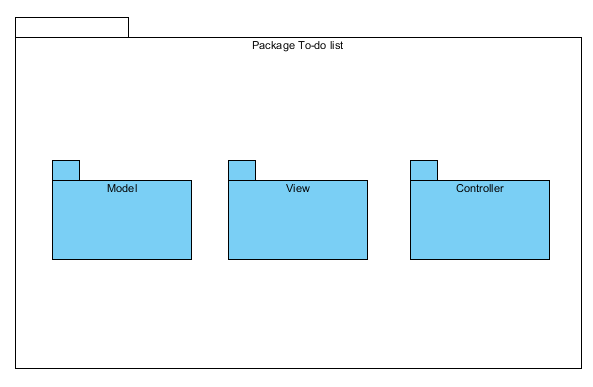
\includegraphics[width=14cm]{../../documenti/SpecificaTecnica/diagrammi_img/classi_e_package/todo.png}
	\caption{Package To-do list}
\end{figure}

\subparagraph{Model}\mbox{}\\
Il package Model gestisce i dati contenuti nella bubble memory e nel database associato tramite i package ItemsStore e DataChecker. Permette inoltre di impostare notifiche tramite il package Notification.  
\begin{figure}[H]
	\centering
	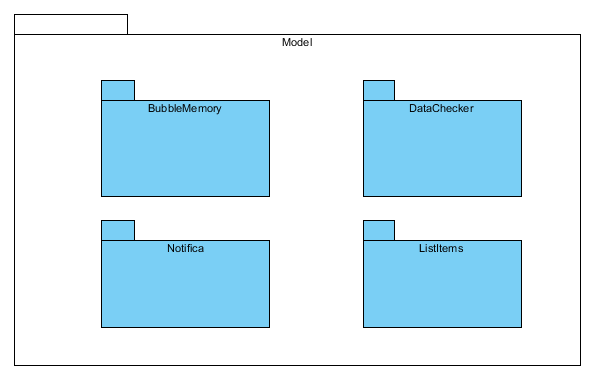
\includegraphics[width=14cm]{../../documenti/SpecificaTecnica/diagrammi_img/classi_e_package/todo_model.png}
	\caption{Model}
\end{figure}

\subsubparagraph{TodoList\-::Model\-::ItemsStore}\label{todo-itemsstore}\mbox{}\\
\textbf{Descrizione:}\\
La classe ItemsStore contiene i dati riguardanti le entrate della TodoList.\\
\textbf{Utilizzo:}\\
L'utilizzo di questa classe è quello di fornire il salvataggio dei dati per le entrate della bubble To-do list in modo da poter modificare i dati alla creazione, eliminazione o completamento di voci della lista.\\
\textbf{Dipendenze:}
\begin{itemize}
	\item \texttt{ListItems::ListItemContainer}: nello store vengono memorizzati uno o più contenitori (liste).
\end{itemize}

\subsubparagraph{TodoList\-::Model\-::Data\-Checker}\label{todo-datachecker}\mbox{}\\
\textbf{Descrizione:}\\
La classe DataChecker verifica la correttezza dei dati rispetto ad uno schema dato e li salva sul database.\\
\textbf{Utilizzo:}\\
Questa classe permette di verificare l'integrità dei dati inviati dall'utente rispetto ad uno schema dato, salvandoli successivamente sul database.

\subsubparagraph{TodoList\-::Model\-::ListItems}\mbox{}\\ \label{todo-item-model}
\begin{figure}[H]
	\centering
	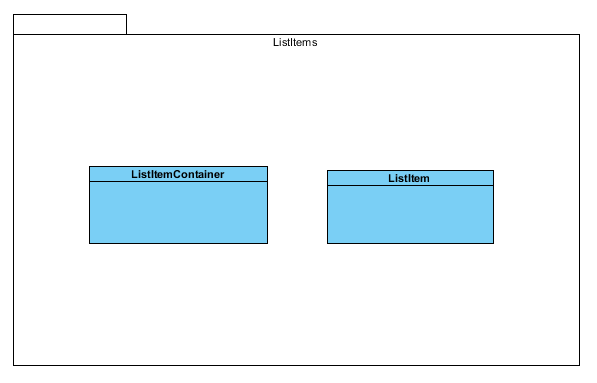
\includegraphics[width=14cm]{../../documenti/SpecificaTecnica/diagrammi_img/classi_e_package/todo_listitems.png}
	\caption{List\-Items}
\end{figure}

Il package ListItems rappresenta tramite le classi che contiene la to-do list a livello logico.\\
\begin{description}
	\item[\textbf{TodoList\-::Model\-::ListItems::ListItem}] \hfill\\
	\textbf{Descrizione:}\\
	La classe ListItem rappresenta una voce della to-do list.\\
	\textbf{Utilizzo:}\\
	Viene utilizzata per contenere i dati relativi alla voce della lista.
	\item[\textbf{TodoList\-::Model\-::ListItems::ListItemContainer}] \hfill\\
	\textbf{Descrizione:}\\
	La classe ListItemContainer rappresenta un contenitore per gli elementi della lista, ovvero la lista stessa.\\
	\textbf{Utilizzo:}\\
	Viene utilizzata per mantenere le informazioni riguardo alla lista.\\
	\textbf{Dipendenze:}
	\begin{itemize}
		\item \texttt{ListItem}: essendo un contenitore, ListItemContainer è una aggregazione di ListItem.
	\end{itemize}
\end{description}


\subparagraph{View}\mbox{}\\
\nopagebreak
\begin{figure}[H]
	\centering
	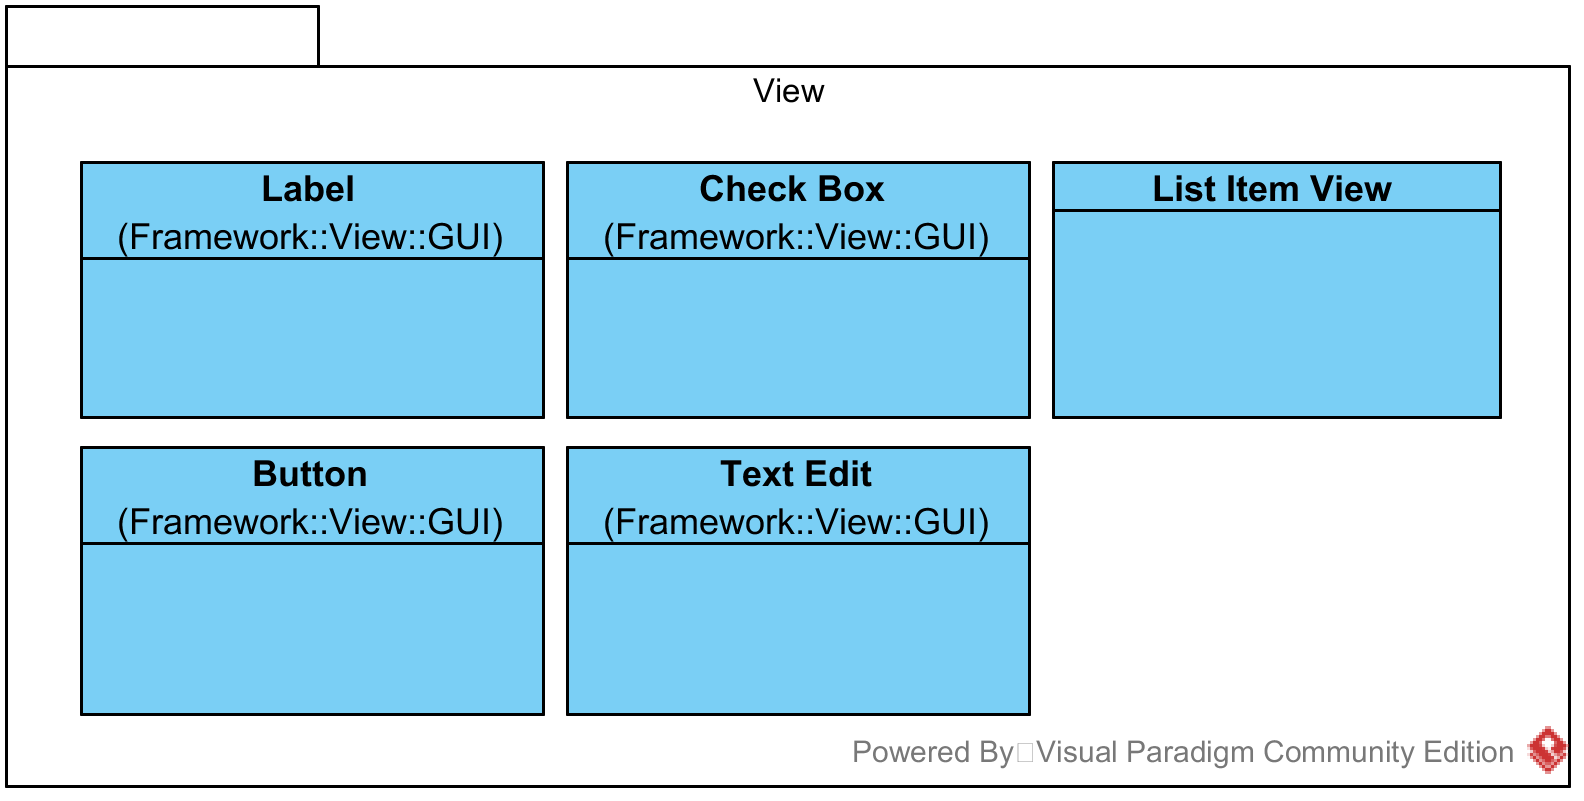
\includegraphics[width=14cm]{../../documenti/SpecificaTecnica/diagrammi_img/classi_e_package/todo_view.png}
	\caption{View}
\end{figure}

\subsubparagraph{TodoList\-::View\-::ListItemView}\label{todo-view}\mbox{}\\
\textbf{Descrizione:}\\
La classe ListItemView rappresenta graficamente un'entrata per la To-do list.\\
\textbf{Utilizzo:}\\
Lo scopo di questa classe è quello di rappresentare le singole entrate della To-do list e permetterne la selezione per la gestione della rimozione e del completamento in modo indipendente dalle altre voci all'interno della lista.\\
\textbf{Dipendenze:}
\begin{itemize}
	\item \texttt{Framework::View::GUI::CheckBox}: checkbox tramite cui è possibile spuntare l'oggetto;
	\item \texttt{Framework::View::GUI::Label}: etichetta di testo per l'elemento.
\end{itemize}
ListItemView può essere esteso utilizzando bottoni e testo editabile come entry.


\subparagraph{Controller}\mbox{}
\begin{samepage}
	\subsubparagraph{TodoList\-::Controller\-::ListItemController}\label{todo-controller}\mbox{}\\
	\nopagebreak
	\begin{figure}[H]
		\centering
		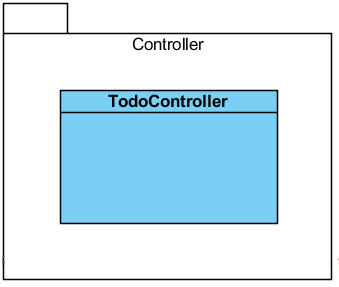
\includegraphics[width=15cm]{diagrammi_img/classi_e_package/todo_controller}
		\caption{Controller\-::ListItemsController}
	\end{figure}
\end{samepage}
\textbf{Descrizione:}\\
La classe ListItemController permette di associare agli elementi della view funzionalità logiche definite nel model.\\
\textbf{Utilizzo:}\\
La funzione di questa classe è quella di Controller della To-do list; essa controlla la renderizzazione grafica ed il comportamento della To-do list.\\
\textbf{Dipendenze:}
\begin{itemize}
	\item \texttt{TodoList::View::ListItemView}: utilizzato per rappresentare graficamente gli elementi della lista;
	\item \texttt{TodoList::Model::ListItemStore}: store per le liste;
	\item \texttt{TodoList::Model::ListItemContainer}: per manipolare la lista.
\end{itemize}
